\subsection{Route Filtering} \label{sec:routefilter}
\begin{figure}[h!] 
	\centering
	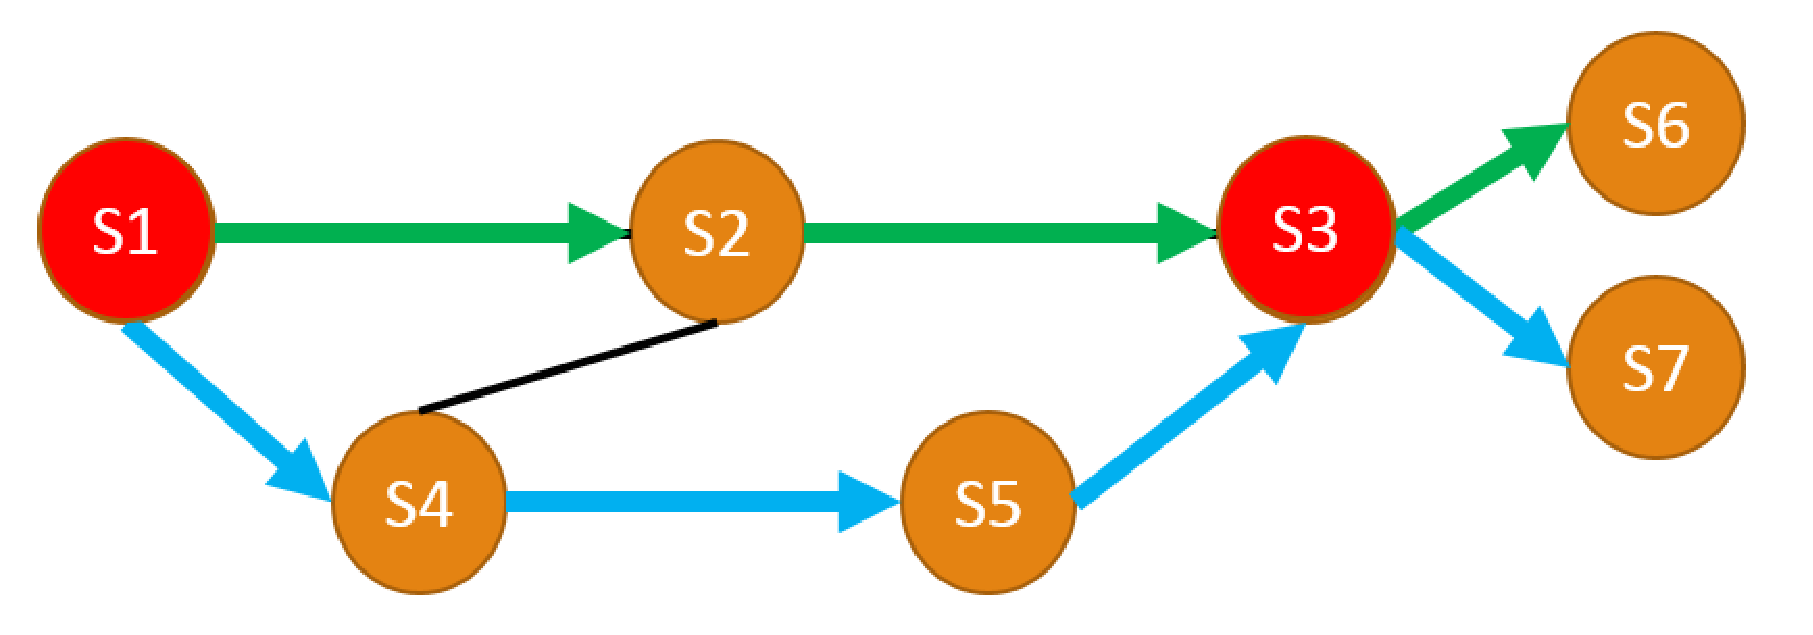
\includegraphics[width=\columnwidth]{figures/diamond.eps}
	\caption{Data plane example which requires route-filtering} \label{fig:diamond}
\end{figure}
Pure ARCs cannot be synthesized for all data planes. Consider the data
plane in \Cref{fig:diamond}. 
There exists no solution to the edge weights for this data plane. This is because 
there are two disjoint shortest paths connecting $s1$ and $s3$, and each path will have 
constraints
asserting it is the shortest of the two paths. 

How can we synthesize an ARC for the above scenario? 
If we could disable the edge
$s1 \rightarrow s4$ for destination $s6$, then we can synthesize ARC weights
such that path $s1 \rightarrow s2 \rightarrow s3$ is taken to reach $s6$, 
even if the actual shortest path
from $s1$ to $s3$ is via $s4$ and $s5$. 
If a route-filter is added on switch $s4$, $s4$ 
will not advertise a route for $s6$ to $s1$, so 
$s1$ will forward to $s2$ and not to $s4$
to reach $s6$. The forwarding of packets destined
for $s7$ are not affected, and they will be sent from
$s1$ to $s4$ as it is the shortest path.
Thus, by incorporating route-filters, we can
disable certain links in the topology 
for specific destinations, and increase the 
expressiveness of our synthesis. \kausik{expressiveness
may not be the right term.}

Given a data plane, we can trivially find an 
ARC enforcing the data plane by placing 
route-filters on all alternate paths ()%\Cref{fig:routefilter})
except the shortest paths of the DAGs. However, this
ARC lacks the resilience properties we desire in
distributed control planes. Moreover, this ARC would be
0-resilient, and a single link failure can sever 
connectivity among endpoints (as all alternate paths
are blocked by route-filters). Thus, our objective is
to pick a subset of the route-filters for each destination
as illustrated by <ref-to-rf-fig> such that the 
ARC satisfies certain properties. For e.g., we can
try to find the optimal number of route-filters such 
that the ARC synthesis succeeds, or we can choose a
subset that maximizes the resilience of each path 
in terms of number of edge-disjoint paths in the ARC
for each endpoint. 

\subsubsection{Linear Equations with Route-Filters}
Given a set of route-filters, we generate a modified 
set of linear equations than the set in \secref{sec:linearequations}
such that the semantics of route-filters is satisfied. 
For convenience, we define $RF(sw_1, sw_2, d) = True$ 
if a route filter disables the link $sw_1 \rightarrow sw_2$
for forwarding to destination $d$ (The route filter will
actually be present on $sw_2$). 

When $RF(sw_1, sw_2, d)$ is set, we can ignore the 
weight of any path using the $sw_1 \rightarrow sw_2$
link for destination $d$, and thus 
the weight of the path of DAG $\xi_d$
starting at $sw_1$ need not be smaller than the path weights
using the the $sw_1 \rightarrow sw_2$ link. Thus,
we prune \Cref{eq:uniq} to enforce the route-filter accordingly:
\begin{multline} \label{eq:uniq}
		\forall d \in \Omega. \forall s, t \in \xi_d. (s \rightarrow^+ t).\\ 
		\forall n'. (n' \in N(s) \wedge n' \not\in N(s, \xi_d) \wedge \neg RF(s,n',d)). \\
		\sum_{\mathclap{\substack{(sw_1, sw_2) \in (s \rightarrow^+ t)}}} 
		E(sw_1, sw_2) < E(s, n') + D(n', t)   
\end{multline}

\subsubsection{Diamond Elimination}
We define the structure shown in \Cref{fig:diamond}
as a \emph{diamond}. Formally,
consider two switches $s$ (the source of the diamond) 
and $t$ (the target of the diamond).
There exist two different destination DAGs with 
paths starting from $s$ such that they forward t
o different switches from $s$  
and these divergent paths from $s$ converge
at the switch $t$ first. A diamond is 
a reason for the ARC synthesis resulting in no
solution. 
\begin{theorem} \label{thm:diamond}
If the data plane contains a diamond, then no pure ARC  
can be synthesized for the data plane.
\end{theorem}
Thus, to generate an ARC, we need route-filters
to eliminate the diamond structures. Consider
the diamond in \Cref{fig:diamond}. There are two choices
of route-filters: the $s1-s2$ edge for destination $s7$ 
and the $s1-s4$ edge for destination $s6$, out of which,
at least one filter is required to eliminate the 
inconsistency in the linear equations due to the diamond.
Thus, we find all diamonds for all pairs of destination
DAGs (this is done in polynomial time) and assign a filter
to one of the two edges at the source of each diamond. 

\subsubsection{Unsat-Core Learning Approach}
The converse of \thmref{thm:diamond} does not hold, i.e.,
there exists data planes without diamonds for which
we cannot synthesize a pure ARC. We illustrate one example
in \Cref{}. (example figure and why inconsistent). 

\kausik{This para may need more work.}
Characterising the properties of structures causing
inconsistencies in the ARC synthesis is a tough algorithmic
problem and is an interesting study of future work. An
efficient algorithm to find the structures causing 
inconsistencies can be used to assign route-filters in an
optimal manner, thus maximizing resilience of the control plane.

Modern LP-solvers have efficient procedures to return an
unsatisfiable core, also called IIS (Irreducible Inconsistent Subsystem)
~\cite{iis}. Formally, an IIS is a subset of constraints such that
if all constraints except those in the IIS are removed, the set of
linear equations is still inconsistent. However, further removing 
any one constraint of the IIS produces an consistent result. 

In the case of the ARC synthesis, suppose we obtain
a unsatisfiable core (unsat-core) from the solver. 
Some linear inequalities 
from \Cref{sec:uniq} would be present in the unsat-core 
(an unsat-core cannot consist only 
inequalities from \Cref{sec:dist}, as all distances set to zero
would trivially be consistent). Each linear inequality
in the unsat-core will be of the form:
\begin{eqnarray}
	\sum_{\mathclap{\substack{(sw_1, sw_2) \in (s \rightarrow^+ t)}}} 
		E(sw_1, sw_2) < E(s, n') + D(n', t)  \nonumber
\end{eqnarray}
If we set $RF(s,n',d) = True$ where the DAG of destination $d$
contains the $s \rightarrow^+ t$, then this inequality would be pruned,
and the set of equations in the unsat-core will be consistent (though
the whole set of equations may still be inconsistent) by the 
irreducible property of the unsat-core. By adding this route-filter
permanently to the ARC, we are assured that this unsat-core will 
never be a cause of inconsistency. Thus, our unsat-core learning
approach uses the unsat-core to learn where to place a route-filter,
and we repeat this process with an updated set of filters till the
set of linear equations are consistent. The complete 
algorithm of finding the set of route-filters is shown 
in Fig <>.

Given an unsat-core, we have a set of route-filters (obtained
from the linear inequalities of \Cref{sec:dist}) of which we 
need to choose one to eliminate this unsat-core. Thus, synthesis 
of the ARC with route-filters can be 
described as follows: given the set of all
unsat-cores for the original set of equations, find a 
set of route-filters such that each unsat-cores are eliminated
by a route-filter in the set. 
We can 
adopt a greedy approach (based on the lines of 
set cover \cite{}) of picking a route-filter which 
eliminates the maximum number of unsat-cores. However, 
finding the number of unsat-cores a route-filter eliminates
is an open problem and instrumental in minimizing the number 
of route-filters.

Alternatively, another scheme we propose in choosing route-filters
is to maximize the number of edge-disjoint paths for each pair of
endpoints in the input data plane, thus maximizing the resilience 
property of the control plane (t+1 edge-disjoint paths indicate
{\em t-resilience}). Thus, when given an unsat-core, we can choose
a route-filter which does not affect the number of edge-disjoint paths
for that pair of endpoints.



